%----------------------------------------------------------------------------------------
%	SECTION 1.1
%----------------------------------------------------------------------------------------

\section{Capacity and Cost.}
\label{section1}

We define now in a more precise manner the discrete memoryless channel.

\begin{definition}
    A \textbf{discrete memoryless channel} is a triple $D=(A_X,A_Y,Q)$, where
    $A_X$ and  $A_Y$ are finite sets of size  $|A_X|=r$ and  $|A_Y|=s$, called
    the \textbf{input alphabet}, and \textbf{output alphabet}, respectively; and
    $Q$ is an  $r \times s$ matrix called the  \textbf{transitional probability
    matrix} whose entries are $(p(y|x))$. We also define a map $b:A_X
    \rightarrow \R$ called the \textbf{cost function} of $D$, and we call the
    value  $b(x)$ the \textbf{cost} of $x$.
\end{definition}

\begin{example}
    \begin{enumerate}
        \item[(1)] Let $A_X=A_Y=\F_2$ with  $Q=\begin{pmatrix} 1-p & p \\ p
            & 1-p \\\end{pmatrix}$, where $0 \leq p \leq \frac{1}{2}$, and
            $b(0)=0$, $b(1)=1$. This describes a DMC called the \textbf{binary
            symmetric channel}.

        \item[(2)] Let $A_X=\{0, \frac{1}{2}, 1\}$ and $A_Y=\F_2$, with
                $Q=\begin{pmatrix} 1 & 0 \\ \frac{1}{2} & \frac{1}{2} \\ 0 &
                1 \\\end{pmatrix}$ with $b(0)=b(1)=1$ and $b(\frac{1}{2})=0$.

        \item[(3)] Let $A_X=A_Y=\F_3$, with  $Q=I_{3 \times 3}$ and
            $b(0)=b(1)=1$ and $b(2)=4$.
    \end{enumerate}
\end{example}

\begin{definition}
    Let $D=(A_X,A_Y,Q)$ be a DMC with cost $b(x)$. Assume that $D$ is used  $n$
    consecutive times with input and output sequences  $x=\{x_i\}_{i=1}^n$ and
    $y=\{y_i\}_{i=1}^n$. The \textbf{memoryless assumption} that $y_i$ is a
    function only of  $x_i$ is defined to be the product
    $\prod_{i=1}^n{p(x_i,x_i)}$. We define the \textbf{cost} of sending $x$ over
    the channel to  be:
    \begin{equation}
        b(x)=\sum_{i=1}^n{b(x_i)}
    \end{equation}
    We define the \textbf{average cost} of sending $x$ to be:
    \begin{equation}
        \bar{b}(x)=E(b(x))=\sum_{i=1}^n{p(x_i)b(x_i)}
    \end{equation}
\end{definition}

\begin{definition}
    For a DMC $D=(A_X,A_Y,Q)$ with cost $b(x_i)$ and $n \in \Z^+$; we define the
     \textbf{$n$-th capacity-cost function} of $D$ to be:
     \begin{equation}
         C_n(\beta)=\max_{x,y \in A_X^n \times A_Y^n}{\{I(X,Y) : \bar{b}(x)\leq
         n\beta\}}
     \end{equation}
     Where $X$ and  $Y$ are the random variables associated with  $x$ and  $y$.
     We call $x$ the \textbf{test source}, and say it is
     \textbf{$\beta$-admissable} if $\bar{b}(x) \leq n\beta$.
\end{definition}

\begin{lemma}\label{3.1.1}
    For a test source $x=\{x_i\}$, if $\beta_{\min}=\min_{x_i \in A_X}{b(x_i)}$,
    then $n\beta_{\min} \leq \bar{b}(x)$.
\end{lemma}
\begin{proof}
    Notice that $\beta_{\min} \leq
    \frac{\sum{p(x_i)b(x_i)}}{n}=\frac{\bar{b}(x)}{n}$.
\end{proof}
\begin{corollary}
    $C_n(\beta)$ is defined for all $\beta \geq \beta_{\min}$.
\end{corollary}
\begin{corollary}
    If $\beta_{\min} \leq \beta_1 \leq \beta_2$, then $C_n(\beta_1) \leq
    C_n(\beta_2)$.
\end{corollary}
\begin{proof}
    Let $C_i=\{I(X,Y) : \bar{b}(x) \leq n\beta_i\}$ for $1 \leq i \leq 2$. Then
    if $x$ achieves  $C_n(\beta_1)$, that is, $I(X,Y)=C_n(\beta_1) \in C_1$ and
    $\bar{b}(x) \leq n\beta_1$, then $\bar{b}(x) \leq n\beta_2$. This makes
    $I(X,Y) \in C_2$. Thus $C_1 \subseteq C_2$ implying $C_n(\beta_1) \leq
    C_n(\beta_2)$.
\end{proof}

\begin{definition}
    Let $D=(A_X,A_Y,Q)$ be a DMC. We define the \textbf{capacity-cost function}
    of $D$ to be:
    \begin{equation}
        C(\beta)=\sup{\frac{C_n(\beta)}{n}}
    \end{equation}
\end{definition}

\begin{theorem}\label{3.1.2}
    For any $DMC$, the  $n$-th capacity-cost,  $C_n(\beta)$ is convex down for
    all $\beta \geq \beta_{\min}$.
\end{theorem}
\begin{proof}
    Let $\alpha_1,\alpha_2 \geq 0$ with $\alpha_1+\alpha_2=1$ and let $\beta_1,
    \beta_2 \geq \beta_{\min}$. Let $x_1$ and $x_2$ be test sources with
    probailities $p_1(x)$ and $p_2(x)$, both achieving $C_n(\beta_1)$ abd
    $C_n(\beta_2)$, respectively. Define $x$ to be the test source with
    probability $p(x)=\alpha_1p_1(x)+\alpha_2p_2(x)$. Then
    $\bar{b}(x)=\sum_{x}{p(x)b(x)}=\alpha_1\sum{p_1(x)b(x)}+\alpha_2
    \sum{p_2(x)b(x)}=\alpha_1\bar{b}(x_1)+\alpha_2\bar{b}(x_2) \leq
    n(\alpha_1\beta_1+\alpha_2\beta_2)$. Additionally, since $I(X,Y)$ is convex
    down, we have:
    \begin{equation*}
        C_n(\alpha_1\beta_1+\alpha_2\beta_2) \geq I(X,Y) \geq
        \alpha_1I(X_1,Y_1)+\alpha_2I(X_2,Y_2)=\alpha_1C_n(\beta_1)+\alpha_2C_n(\beta_2)
    \end{equation*}
\end{proof}

\begin{theorem}\label{3.1.3}
    For any DMC, $C_n(\beta)=nC_1(\beta)$, for $n \in \Z^+$ and all  $\beta \geq
    \beta_{\min}$.
\end{theorem}
\begin{proof}
    Let $x=\{x_i\}$ be $\beta$-admissable, achieving  $C_n(\beta)$. By theorem
    \ref{2.2.2}, $I(X,Y) \leq \sum{I(X_i,Y_i)}$. Defining $\beta_i=\bar{b}(x_i)$,
    we get $\sum{\beta_i}=\sum{\sum{p(x_i)b(x_i)}}=\bar{b}(x) \leq n\beta$. We
    also have $I(X_i,Y) \leq C_1(\beta_i)$. Then, by Jensen's inequality:
    \begin{equation*}
        \frac{1}{n}\sum{C_1(\beta_i)} \leq
        C_1(\frac{1}{n}\sum{\beta_i})=C_1(\frac{\bar{b}(x)}{n}) \leq C_1(\beta)
    \end{equation*}
    So $C_1$ is increasing, and $\sum{C_1(\beta_i)} \leq nC_1(\beta)$. Then we
    get from the above results, that $C_n(\beta) \leq nC_1(\beta)$.

    Now, let $x=\{x_i\}$ be a $\beta$-admissable test source achieving
    $C_1(\beta)$; i.e. $\bar{b}(x) \leq \beta$, and $I(X,Y)=C_1(\beta)$. Now,
    consider the random variables $X_1, \dots, X_n$, corresponding to $x_1,
    \dots, x_n$ and assume they are independent and identically distributed with
    distributions that of $X$, associated with  $x$. Then
    $\bar{b}(x)=\sum{\bar{b}(x_i)} \leq n\beta$ and
    $I(X,Y)=\sum{I(X_i,Y_i)}=nC_1(\beta)$. This makes $C_n(\beta) \geq
    nC_1(\beta)$.
\end{proof}
\begin{corollary}
    For a memoryless channel, $C(\beta)=C_1(\beta)$.
\end{corollary}

\begin{lemma}\label{3.1.4}
    For all $\beta \geq \beta_{\min}$ $C(\beta)$ is constant for $\beta$
    sufficiently large.
\end{lemma}
\begin{proof}
    Define $C_{\max}=\max{\{C(\beta) : \beta \geq \beta_{\min}\}}=
    \max_{x \in A_X}{\{I(X,Y)\}}$. Define:
    \begin{equation*}
        \beta_{\max}= \min{\{\bar{b}(x) : I(X,Y)=C_{\max}\}}
    \end{equation*}
    Then $C(\beta)=C_{\max}$ for $\beta \geq \beta_{max}$,
    and $C(\beta) < C_{\max}$ otherwise.
\end{proof}

\begin{definition}
    For any $DMC$ $D$, we definie the \textbf{channel capacity} of $D$ to be:
    \begin{equation}
        C_{\max}=\max{\{C(\beta) : \beta \geq \beta_{\min}\}}
    \end{equation}
\end{definition}

\begin{lemma}\label{3.1.5}
    A test source $x$ is  $\beta_{\min}$-admissable if, and only if $p(x)=0$
    whenever $b(x)>\beta_{\min}$.
\end{lemma}

\begin{example}
   Consider the BSC, that is, the triple $(\F_2,\F_2,Q)$ where
    $Q=\begin{pmatrix} 1-p & p \\ p & 1-p \\\end{pmatrix}$, with $0 \leq p \leq
    \frac{1}{2}$ and costs $b(0)=0$ and $b(1)=1$. Then $\beta_{\min}=0$, and the
    reduced channel has only one input, so $C_{\min}=C(0)=0$. Now, let $x$ be a
    test source achieving  $C(\beta)$ for $0 \leq \beta \leq \beta_{\max}$. Then
    $p(1)=\beta$ and $p(0)=1-\beta$, and
    $C(\beta)=H(Y)-H(X|Y)=H((1-\beta)(1-p)+\beta p)-H(p)$. Then $H((1-\beta)
    (1-p)+\beta p)$ attains maximum at $\beta=\frac{1}{2}$, so
    $\beta_{\max}=\frac{1}{2}$. So, $C(\beta)$ gives the curve:
    \begin{equation*}
        C(\beta)=\begin{cases}
                H((1-\beta)(1-p)+\beta p)-H(p), 0 \leq \beta < \frac{1}{2} \\
                \log{2}-H(p), \beta \geq \frac{1}{2}
             \end{cases}
    \end{equation*}
    \begin{figure}[h]
        \centering
        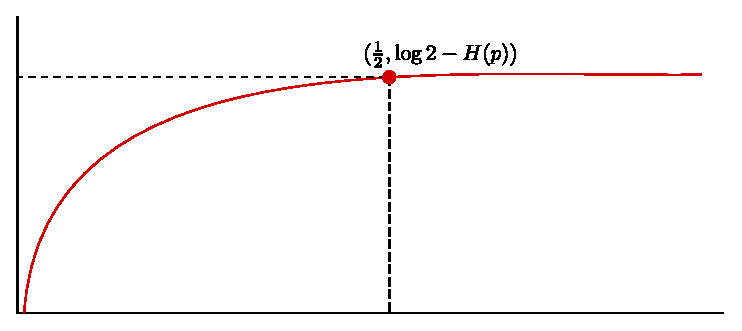
\includegraphics[scale=0.5]{Figures/Chapter3/cap_cost_1.eps}
        \caption{The Capacity-Cost function of the BSC, $C(\beta)$.}
        \label{fig_3.1}
    \end{figure}
\end{example}

\begin{definition}
    We call a $DMC$  $D$ with transition matirx $Q$ symmetric if $Q$ is a
    symmetric matrix.
\end{definition}

\begin{theorem}\label{3.1.6}
    If $D$ is a DMC with  $r$ inputs and  $s$ outputs, then the channel capacity
    for  $D$ is a acheived with equiprobable inputs at:
    \begin{equation}
        C_{\max}=\log{s}-H(q_0, \dots, q_{s-1})
    \end{equation}
    where $(q_1 \ \dots \ q_{s-1})$ is any row of the transition matrix $Q$ of $D$.
\end{theorem}
\begin{proof}
    We have $I(X,Y)=H(Y)-H(Y|X)=H(Y)-\sum_{x}{p(x)H(Y|x)}$. Now,
    \begin{equation*}
        H(Y|x)=\sum_{y}{p(y|x)\log(\frac{1}{p(y|x)})}=H(q_0, \dots q_{s-1})
    \end{equation*}
    is independent of $X$, so by theorem \ref {2.1.2}, $H(Y) \leq \log{s}$, with
    equality holding if, and only if $p(y)=\frac{1}{s}$ for all $y \in A_Y$.
    This is implied by the transition matrix, and so gives us the result.
\end{proof}

\begin{example}
       \begin{enumerate}
           \item[(1)] Consider a DMC with transition matrix
            $Q=\begin{pmatrix}
                    \frac{1}{3} & \frac{1}{3} & \frac{1}{6} & \frac{1}{6} \\
                    \frac{1}{6} & \frac{1}{6} & \frac{1}{3} & \frac{1}{3} \\
               \end{pmatrix}$
            then, the DMC has channel capacity $C_{\max}=\log{4}-H(\frac{1}{3},
            \frac{1}{3}, \frac{1}{6}, \frac{1}{6})=\log{\frac{\sqrt[3]{2^5}}{3}}$
            bits.

        \item[(2)] Consider the \textbf{r-ary symmetric channel} with transition
            $r \times r$ matrix $(q_{xy})$ where $q_{xy}=\epsilon$ if $x \neq y$
            and  $q_{xy}=1-(r-1)\epsilon$ otherwise. For $r=2$, we get the BSC,
            and for $r=4$, we get
            \begin{equation*}
                Q=\begin{pmatrix}
                    1-3\epsilon & \epsilon & \epsilon & \epsilon \\
                    \epsilon & 1-3\epsilon & \epsilon & \epsilon \\
                    \epsilon & \epsilon & 1-3\epsilon & \epsilon \\
                    \epsilon & \epsilon & \epsilon & 1-3\epsilon \\
                  \end{pmatrix}
            \end{equation*}
            The channel capacity for this channel is $\log{r}-H(1-(r-1)\epsilon,
            \epsilon, \epsilon, \epsilon)=\log{r}+(1-r)\epsilon\log{\epsilon}+
            (1-r\epsilon+\epsilon)\log{(1-r\epsilon+\epsilon)}$.
       \end{enumerate}
\end{example}
